\section{Opis implementacji}
Programy wykorzystane w danej pracy zostały napisane w Pythonie. Wszystkie wykorzystywane zbiory pochodzą z witryny Kaggle \cite{kaggle_site}. Na niej też znaleziono prace, którymi wzorowano się przetwarzając dane. Przetworzony i podzielony na podzbiory zbiór jest poddawany nauce przez jeden z modeli. Wynikiem takiej operacji są miary, macierz pomyłek oraz (w przypadku dancyh w postaci zdjęć) prawdopodobieństwa przynależności do poszczególnych klas dla wskazanej próbki. Ów model poddawany jest analizie poprzez metodę XAI. Następnie wykorzystywana jest kolejna metoda. Po użyciu 3 metod uczony i analizowany jest kolejny model. Na danych tabelarycznych do nauki wykorzystywane są Random Forest, XGBoost oraz sieć neuronowa, a wyjaśniane są one przez LIME, SHAP i PFI. W przypadku zbiorów składających się z obrazów - używane modele to: VGG-16, ResNet50 i Xception. Ich analizą zajmują się LIME, SHAP oraz Grad-CAM. 

Random Forest \cite{rfc_documentation} oraz sieć neuronowa \cite{mlpc_documentation} pochodzą z biblioteki scikit-learn (sklearn). XGBoost \cite{xgb_documentation} jest oddzielnym modułem, którego biblioteka nosi nazwę ,,xgboost''. VGG-16 \cite{vgg16_documentation}, ResNet50 \cite{resnet50_documentation} i Xception \cite{xception_documentation} są częścią biblioteki Keras, której frameworkiem backendowym był TensorFlow w wersji 2.20.0 \cite{tensorflow_site}. Przestrzeń przykładowych rozwiązań została przeszukana za pomocą funkcji ,,GridSearchCV'', znajdując optymalne parametry sieci neuronoweych \cite{gridsearchcv_documentation}. Na modelach CNN został przeprowadzony \textit{fine tuning}. Bazowe wagi zostały ,,zamrożone'', a na końcu dodano warstwy \textit{Flatten} (w kontekście zbioru dotyczącego zmian nowotworowych mózgu) lub \textit{GlobalAveragePooling2D} (zbiór dotyczący psów i kotów) i \textit{Dropout}. W przypadku zbioru dotyczącego wykrywania zmian nowotworowych w mózgu wagi do modeli VGG-16 oraz Xception również pochodzą ze strony Kaggle \cite{kaggle_pretrain_models}. 

Modele oceniono na podstawie metryk, które możemy znaleźć w pakiecie biblioteki scikit-learn. ,,roc\_auc\_score'' to funkcja obliczająca pole pod krzywą ROC na podstawie osiągniętych predykcji. W przypadku zbioru dotyczącego choroby serca, który jest problemem wieloklasowym, w parametrach wejściowych podano zmienną ,,multi\_class'' równą ,,ovr'' oraz ,,average'' - ,,macro''. Pierwsza z nich oznacza, że AUC będzie obliczana w sposób jedna klasa przeciwko wszystkim innym, czyli będzie uznana za pozytywną, a reszta - negatywną \cite{roc_ovr_documentation}. Druga, że wyniki zostaną uśrednione za pomocą średniej arytmetycznej \cite{roc_auc_score_documentation}. Precyzja, czułość, F1-score, liczebność, dokładność oraz średnie arytmetyczne i ważone zostały obliczone poprzez ,,classification\_report'' \cite{classification_report_documentation}. Macierz pomyłek została stworzona przy pomocy ,,confusion\_matrix'' \cite{confusion_matrix_documentation}.

Metodę LIME zaimportowano z biblioteki o takiej samej nazwie \cite{lime_documentation}. Tworząc część dla danych tabelarycznych skorzystano z wpisu na stronie GeekForGeeks \cite{lime_tabular_code}, filmu zamieszczonego na platformie YouTube \cite{lime_yt_video} oraz dokumentacji. Dwoma najważniejszymi funkcjami są ,,LimeTabularExplainer'' oraz ,,explain\_instance''. Ta pierwsza pozwala na~stworzenie obiektu do predykcji próbek, a druga tworzy tłumaczenie jednego konkretnego przypadku. Pisząc wersję do obrazów wykorzystano fragmenty kodu znajdujące się w poradniku stworzonym przez twórcę biblioteki \cite{lime_images_code}. Tutaj użyto ,,LimeImageExplainer'', które działa analogicznie do tego, używanego przy rekordach tabel oraz ,,explain\_instance''. W obydwu przypadkach zmodyfikowano kody, tak, aby działały z wykorzystywanymi danymi oraz ich niektóre linie wykonywały się w pętli.

Biblioteka ,,shap'' pozwoliła na skorzystanie z kolejnej metody. Jej dokumentacja \cite{shap_documentation} oraz film zamieszczony na platformie YouTube \cite{shap_yt_video} znacznie pomogły w pisaniu kodu do~tabelarycznych zbiorów. Jedną z najważniejszych jego części jest funkcja ,,get\_explainer'', w której znajduje się metoda ,,shap.Explainer'' pozwalająca na stworzenie obiektu tłumaczącego model. Ze względu na format danych wejściowych, jaki jest przez nią wymagany, znajduje się tam instrukcja warunkowa oparta o nazwę przekazanego modelu, która przekazuje odpowiednie zmienne. Sama metoda potrafi własnoręcznie wybrać odpowiedni rodzaj obiektu wyjaśniającego, w tym ,,shap.TreeExplainer'' i ,,shap.DeepExplainer''. Część programu do danych będących obrazami jest jednym z przykładów znajdujących się na stronie z dokumentacją \cite{shap_image_documentation}. Najpierw tworzony jest w niej masker, następnie obiekt objaśniający, któremu przekazywana jest badana próbka. Zwraca on wartości końcowo prezentowane za~pomocą funkcji ,,shap.image\_plot''.

PFI jest jedną z funkcji biblioteki scikit-learn pakietu ,,inspection''. Na stronie dedykowanej właśnie jej można znaleźć przydatne kody wykorzystujące metodę, tworząc przy tym proste, zrozumiałe wyniki. Fragment programu stworzony na rzecz omawianego zagadnienia jest połączeniem dwóch znajdujących się na tej witrynie \cite{pfi_documentation, pfi_example}. Najważniejszą jego częścią jest wywołanie funkcji ,,permutation\_importance'' odpowiadającej za wykonanie metody PFI i zwrócenie jej wyników \cite{permutation_importance_function}. Takie dane są sortowane malejąco po uzyskanym średnim wpływie na dokładność i wypisywane na ekran. Następnie na ich podstawie tworzona jest tabela, której zawartość zostaje umieszczona na wykresie.

Implementując metodę Grad-Cam użyto kodu znalezionego na stronie dedykowanej bibliotece Keras \cite{grad-cam_code}. Został on przerobiony w taki sposób, aby pozwalał na~wykorzystanie używanych w pracy danych i różnych modeli. Najważniejszą częścią kodu jest funkcja ,,make\_gradcam\_heatmap'', w której najpierw pobierany jest model bazowy. Później tworzony jest nowy model łączący wejściowy obraz z wyjściami wskazanej warstwy konwolucyjnej (ostatniej). Następnie odtwarzana jest struktura powstała na skutek dostrajania, a~na~jej podstawie powstają gradienty i mapa cieplna.

\subsection{Analizowane zbiory}
Zbiór danych \textbf{,,Diabetes Prediction''} jest binarnym problemem klasyfikacyjnym polegającym na przewidzeniu, czy dana osoba posiada cukrzycę. Składa się z 22 kolumn i ponad 250 000 rekordów. Zmienną docelową jest w nim 'Diabetes\_binary' mówiąca o braku (,,0'') lub występowaniu choroby (,,1''), dane objaśniające zostały zawarte w tabeli \ref{tab:explanatory_var_diabetes} \cite{diabetes_dataset}.   


\begin{xltabular}{\textwidth}{| c | >{\centering\arraybackslash}X | c |}
\caption{Zmienne objaśniające zbioru dotyczącego diabetyków}
\label{tab:explanatory_var_diabetes}\\
\hline
Cecha & Opis & Wartości \\ \hline
\endfirsthead

HighBP & dorośli, którzy usłyszeli od personelu medycznego, że mają wysokie ciśnienie krwi & ,,0'' - nie, ,,1'' - tak \\ \hline
HighChol & osoby, które kiedykolwiek usłyszały od personelu medycznego, iż mają wysoki poziom cholesterolu we krwi & ,,0'' - nie, ,,1'' - tak \\ \hline
CholCheck & czy w przeciągu ostatnich 5 lat sprawdzony został poziom cholesterolu? & ,,0'' - nie, ,,1'' - tak \\ \hline
BMI & wskaźnik masy ciała & 12 - 98 \\ \hline
Smoker & czy wypaliłeś(-łaś) co najmniej 100 papierosów w swoim życiu? & ,,0'' - nie, ,,1'' - tak \\ \hline
Stroke & czy kiedykolwiek miałeś (-aś) udar mózgu? & ,,0'' - nie, ,,1'' - tak \\ \hline
HeartDiseaseorAttack & czy kiedykolwiek zgłoszona została choroba wieńcowa lub zawał mięśnia sercowego? & ,,0'' - nie, ,,1'' - tak \\ \hline
PhysActivity & czy w przeciągu ostatnich 30 dni przeprowadzana była jakakolwiek aktywność fizyczna niezwiązana z wykonywaną na co dzień pracą? & ,,0'' - nie, ,,1'' - tak \\ \hline
Fruits & czy przynajmniej raz dziennie spożywany jest owoc? & ,,0'' - nie, ,,1'' - tak \\ \hline
Veggies & czy przynajmniej raz dziennie spożywane jest warzywo? & ,,0'' - nie, ,,1'' - tak \\ \hline
HvyAlcoholConsump & osoby dużo pijące, do których zalicza się mężczyzn spożywających więcej niż 14 drinków tygodniowo oraz kobiety spożywające więcej niż 7 drinków tygodniowo & ,,0'' - nie, ,,1'' - tak \\ \hline
AnyHealthcare & czy posiadasz ubezpieczenie zdrowotne? & ,,0'' - nie, ,,1'' - tak \\ \hline
NoDocbcCost & czy w przeciągu ostatniego roku zdarzyła się sytuacja, w której potrzebna tobie była opieka zdrowotna, ale nie mogłeś (-aś) z niej skorzystać ze względu na koszty? & ,,0'' - nie, ,,1'' - tak \\ \hline
GenHlth & na ile oceniasz swoje zdrowie? & 1 - 5 \\ \hline
MentHlth & biorąc pod uwagę stres, depresję oraz problemy z emocjami przez ile dni w przeciągu ostatnich 30 twoje zdrowie psychiczne nie było w dobrym stanie? & 0 - 30 \\ \hline
PhysHlth & biorąc pod uwagę choroby fizyczne i kontuzje ile dni w przeciągu ostatnich 30 twój stan fizyczny nie był dobry? & 0 - 30 \\ \hline
DiffWalk & czy masz poważne problemy z wchodzeniem po schodach lub chodzeniem? & ,,0'' - nie, ,,1'' - tak \\ \hline
Sex & płeć & ,,0'' - kobieta, ,,1'' - mężczyzna \\ \hline
Age & wiek respondenta zapisany jako 1 z 14 kategorii & 1 - 14 \\ \hline
Education & jakie jest twoje najwyższe wykształcenie lub ukończony rok szkoły & 1 - 6 \\ \hline
Income & dochód respondenta należący do jednej z 8 kategorii & 1 - 8 \\ \hline
\end{xltabular}

\begin{figure}[H]
    \centering
    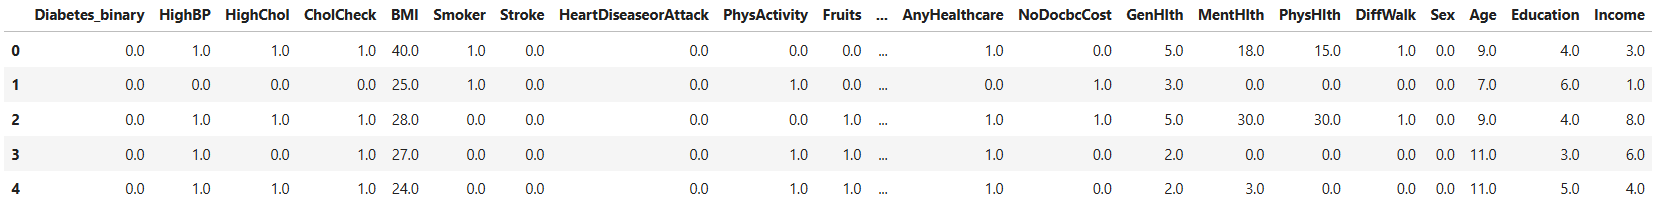
\includegraphics[width=1\linewidth]{rysunki/diabetes/diabetes_data.png}
    \caption{Wykaz 5 pierwszych rekordów zbioru dotyczącego diabetyków [źródło własne]}
    \label{fig:diabetes_data}
\end{figure}

Zbiór nie zawierał braków, a wszystkie zawarte w nim dane były nominalne. Zgodnie z opisem większość cech jest zerem lub jedynką. Najwięcej unikalnych wyników możemy znaleźć w kolumnie 'BMI'. Badania nie wykazały jakichkolwiek wartości odstających, jednak pojawiły się duplikaty, które zostały usunięte. Mapa cieplna oraz VIF nie wskazały, aby pomiędzy którymikolwiek cechami zachodziła znaczna współliniowość (założony próg 0.85). Po przeanalizowaniu histogramów można zauważyć, że dane nie mają rozkładu normalnego. W ramach zbadania istotności zmiennych użyto testu U-Manna Whitneya, z~którego nie wynikło, aby w zbiorze znajdywały się nadmiarowe informacje. Po wykonaniu tych operacji składał się on z prawie 230 000 rekordów, co znacznie wpłynęłoby na~czas potrzebny do przeprowadzenia badań. W związku z tym losowo wybrano po 2 500 wierszy z~obu klas decyzyjnych i połączono je w jeden zestaw danych. Został on podzielony na zbiór treningowy i testowy w stosunku 4:1 z użyciem opcji ,,stratify'' pozwalającej na~rozdzielenie rekordów w taki sposób, aby w obydwu podzbiorach znalazła się równa ilość danych z~poszczególnych klas. Następnie dokonano standaryzacji zmiennych objaśniających stosując średnią oraz odchylenie standardowe uzyskane na próbkach przeznaczonych do nauki \cite{diabetes_dataset_preprocessing}.\\

\textbf{,,UCI Heart Disease Data''}, to drugi analizowany zbiór danych. Dotyczy on występowania choroby serca oraz jej nasilenie, co czyni go problemem klasyfikacji wieloklasowej. Zawiera 16 kolumn oraz 920 rekordów. ,,Id'' jest identyfikatorem pacjenta i nie będzie brane pod uwagę podczas badań. Zmienne wejściowe zostały przedstawione w Tabeli \ref{tab:explanatory_var_heart}. Zmienną docelową jest „num”, która oznacza stadium choroby serca. Może ona przyjmować jedną z 5 wartości, gdzie ,,0'' symbolizuje brak problemów z narządem, a ,,4'' poważne trudności \cite{heart_disease_dataset}.

\begin{xltabular}{\textwidth}{|c|>{\centering\arraybackslash}X|>{\centering\arraybackslash}X|}
\caption{Zmienne objaśniające zbioru dotyczącego występowania choroby serca}
\label{tab:explanatory_var_heart}\\

\hline
Cecha & Opis & Wartości \\ \hline
\endfirsthead

age & wiek & 28 - 77 \\ \hline
sex & płeć & ,,Male''/,,Female'' \\ \hline
dataset & miejsce badania & ,,Cleveland''/,,Hungary''/,,VA Long Beach''/,,Switzerland'' \\ \hline
cp & typ bólu klatki piersiowej & ,,asymptomatic''/,,non anginal''/,,atypical angina''/,,typical angina'' \\ \hline
trestbps & spoczynkowe ciśnienie krwi & 0 - 200 \\ \hline
chol & cholesterol całkowity w surowicy & 0 - 603 \\ \hline
fbs & czy poziom cukru we krwi na czczo jest wysoki & ,,FALSE''/,,TRUE'' \\ \hline
restecg & wynik elektrokardiograficzny w spoczynku & ,,normal''/,,st-t abnormality''/,,lv hypertrophy'' \\ \hline
thalch & osiągnięte maksymalne tętno & 60 - 202 \\ \hline
exang & dławica piersiowa wywołana wysiłkiem fizycznym & ,,FALSE''/,,TRUE'' \\ \hline
oldpeak & obniżenie odcinka ST wywołane wysiłkiem fizycznym w porównaniu do spoczynku & -2.6 - 6.2 \\ \hline
slope & spadek odcinka ST podczas szczytowego wysiłku fizycznego & ,,up''/,,downsloping''/,,upsloping'' \\ \hline
ca & liczba głównych naczyń zabarwionych fluoroskopią & 0 - 3 \\ \hline
thal & wynik badania talasemii & ,,normal''/,,fixed defect''/,,reversable defect'' \\ \hline

\end{xltabular}

\begin{figure}[H]
    \centering
    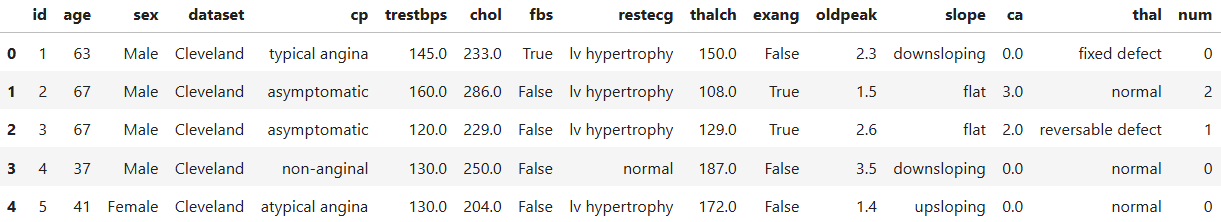
\includegraphics[width=1\linewidth]{rysunki/heart/heart_disease_data.png}
    \caption{Wykaz 5 pierwszych rekordów zbioru dotyczącego występowania choroby serca [źródło własne]}
    \label{fig:heart_disease_5_first_records}
\end{figure}

W trakcie analizy zbioru odkryto, że znajduje się w nim wiele danych brakujących. Najwięcej braków występuje w kolumnie ,,ca''\ - aż 611, co stanowi 66,41\% całości. Dodatkowo zauważono, iż cholesterol w surowicy (,,chol'') nie może przyjąć wartości 0. Takie przypadki również uznano za ubytki. Postanowiono usunąć te kolumny, w których procent owych wartości przekroczył połowę, czyli ,,ca'' oraz ,,thal''. Resztę uzupełniono średnią (zmienne numeryczne) oraz medianą (zmienne kategoryczne). Dane tekstowe zostały zakodowane za pomocą \textit{Label Encoding}'u \cite{heart_disease_dataset_labelencoder}. Po obejrzeniu wyników wykresów pudełkowych, rozstępu międzykwartylowego (IQR) oraz miary z-score zdecydowano się pominąć w tych badaniach rekordy o indeksach: 632, 754, 547. 632 - osiągnięte maksymalne tętno (tutaj 60) jest znacznie niższe od średniej (dla osób w wieku 50 lat wynosi 170 uderzeń na minutę). Ten rekord nie pojawia się we wszystkich testach, aczkolwiek, mimo wszystko, zostanie usunięty. 754 - spoczynkowe ciśnienie krwi nie może wynieść 0, oznaczałoby to śmierć. Prawdopodobnie wartość była liczona, gdy pacjent trafił do szpitala, co jest teoretycznie możliwe, gdyby w tamtym momencie miał zatrzymanie akcji serca i udałoby się go uratować. Inną możliwością jest to, że osobnikowi przy przyjęciu nie zmierzono ciśnienia i wpisano daną wartość. 547 - cholesterol w surowicy osiągający 603 mg/dl, to wynik ekstremalnie wysoki \cite{heart_disease_dataset_chol_mean}. Badanie mapą cieplną wykazało silną korelację (założony próg wynosi 0.85) na poziomie 0.95 pomiędzy identyfikatorem a numerem zbioru, z którego dane pochodziły. Pierwsza z tych cech nie będzie brana pod uwagę w dalszych analizach, co skutkowało brakiem jakichkolwiek zmian. Dane nie mają rozkładu normalnego, więc zmienne zbadano za pomocą testu Kruskala-Wallisa. Wykazał on brak różnic istotnych statystycznie dla ,,restecg'', którego wartość $p$ była większa od założonego progu (0.07106 > 0.05). Dodatkowo istnieje duże niezbilansowanie dotyczące przynależności osób do konkretnych klas. Oznacza to, że jest znacznie mniej przypadków zakwalifikowanych z czwartym stadium choroby niż osób bez przypadłości. Na koniec, po podziale danych na zbiór testowy i treningowy w stosunku 4:1 dokonano standaryzacji zmiennych obu podzbiorów używając średniej oraz odchylenia standardowego uzyskanego na tym, wykorzystywanym do nauki.\\

\textbf{,,Brain MRI Images for Brain Tumor Detection''} jest zbiorem danych zawierającym 253 obrazy rezonansów magnetycznych mózgów. Na jego podstawie można przeprowadzać klasyfikację polegającą na wykrywaniu guzów. 155 zdjęć znajduje się w folderze ,,yes'' oznaczającym wykrycie patologii, reszta została umieszczona w katalogu ,,no'' \cite{brain_dataset}. W dalszej części rozdziału próbki bez zmian nowotworowych będą określane jako klasa ,,0'', a te z - ,,1''. Na Rys. \ref{fig:6_no_brain_tumor} i \ref{fig:6_yes_brain_tumor} znajduje się po 6 przykładowych fotografii z obu klas decyzyjnych. Zauważamy na nich, że obrazy są czarno-białe, a zmiany nowotworowe to białe plamy bądź miejsca o nieregularnych kształtach posiadające obwódkę w tym kolorze.

\begin{figure}[H]
    \centering
    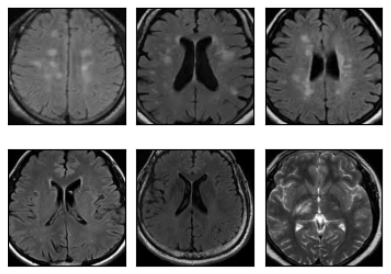
\includegraphics[width=0.5\linewidth]{rysunki//brain/brain_no.png}
    \caption{Sześć przykładowych obrazów bez zmian nowotworowych [źródło własne]}
    \label{fig:6_no_brain_tumor}
\end{figure}

\begin{figure}[H]
    \centering
    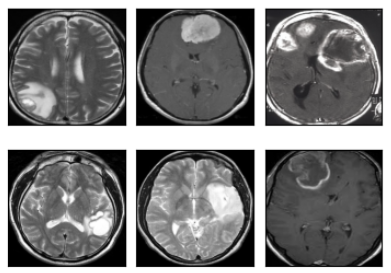
\includegraphics[width=0.5\linewidth]{rysunki//brain/brain_yes.png}
    \caption{Sześć przykładowych obrazów ze zmianami nowotworowymi [źródło własne]}
    \label{fig:6_yes_brain_tumor}
\end{figure}

Na początku stworzono 3 foldery o nazwach "'TRAIN"', "'VAL"' i "'TEST"', w których znalazły się odpowiednio obrazy do nauki, walidacji i testu. 10\% pierwszych plików z obydwu klas decyzyjnych trafiało do zbioru testowego, kolejne 15\% do walidacyjnego, a reszta - treningowego. Następnie je przerobiono wykorzystując kod przycinający zdjęcia do wykrytego konturu głowy dodatkowo je zmniejszając lub powiększając do rozmiaru 224 x 224 pikseli. Takie fotografie zostały przekopiowane do nowoutworzonej analogicznej struktury katalogów w folderze przeznaczonym na przetworzone zbiory. Do nauki modeli użyto augmentacji danych \cite{brain_dataset_preprocessing}. Badana próbka została przedstawiona na Rys. \ref{fig:tested_sample_brain}. Pochodzi ona ze~zbioru treningowego i jest zamieszczona pod indeksem o numerze 94. Wybrano ją ze~względu na~wyraźnie widoczną zmianę nowotworową i jej duże podobieństwo do większości innych analizowanych obrazów.

\begin{figure}[H]
    \centering
    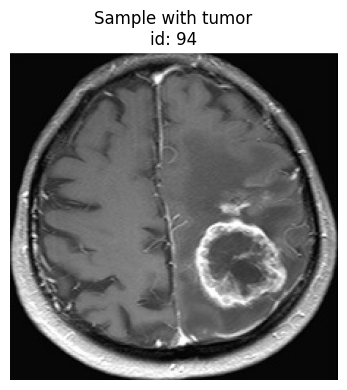
\includegraphics[width=0.3\linewidth]{rysunki/brain/tested_sample_brain.png}
    \caption{Zdjęcie badanej próbki pochodzące ze zbioru dotyczącego zmian nowotworowych mózgu [źródło własne]}
    \label{fig:tested_sample_brain}
\end{figure}

Ostatni analizowany zbiór danych, to \textbf{,,Cats and Dogs Classification Dataset''}. Składa się z 12 499 zdjęć kotów i tylu samo psów, dając łącznie 24 998 próbek. Jest przeznaczony do klasyfikacji binarnej, gdzie klasa ,,0'' oznacza obrazy mruczków, a ,,1'' piesków \cite{cats&dogs_dataset}. Na Rys. \ref{fig:cats&dogs_data} zaprezentowanych zostało 5 przykładowych zdjęć ze zbioru treningowego reprezentujących przedstawicieli obu klas decyzyjnych. Jak można zauważyć, są to obrazy kolorowe, które zostały już przycięte do rozmiaru 224 x 224 pikseli.

\begin{figure}[H]
    \centering
    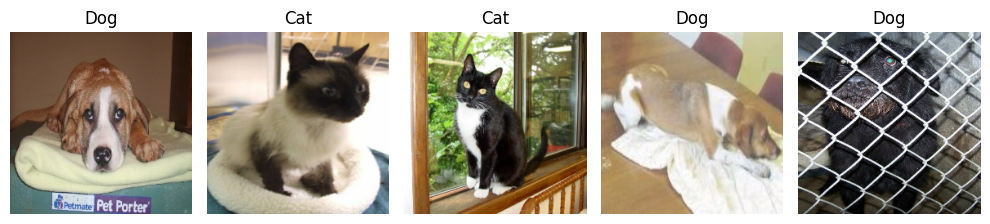
\includegraphics[width=1\linewidth]{rysunki/cats&dogs/cats&dogs_data.png}
    \caption{5 przykładowych zdjęć z podzbioru testowego zbioru dotyczącego klasyfikacji psów i kotów [źródło własne]}
    \label{fig:cats&dogs_data}
\end{figure}

W ramach procesu przygotowania danych, podobnie jak w przypadku poprzedniego zestawu danych, utworzono 3 foldery w folderze przeznaczonym na przetworzone zbiory o~nazwach "'TRAIN"', "'VAL"' i "'TEST"', do których trafiły odpowiednio obrazy do nauki, walidacji i testu. Pierwszy podział dzielił zbiór w stosunku 4:1, z czego ta mniejsza część została przeznaczona na walidację. Druga została poddana ponownemu rozdzieleniu w takiej samej proporcji, przy czym większy podzbiór został zbiorem treningowym, a reszta - testowym. W taki sposób na naukę przypadło 7 999 obrazów przynależących do poszczególnych klas decyzyjnych, po 2 500 do walidacji i po 2 000 do testu. Później przekopiowano je do~odpowiednich katalogów. Zostały wczytane do programu za pomocą funkcji pozwalającej na ich przycięcie do wymaganego przez modele rozmiaru 224 x 224 pikseli. Okazało się, że jedno ze zdjęć z folderu dotyczącego kotów, o nazwie "10404.jpg", ma błędny format, więc zostało pominięte podczas tych badań. Ze względu na użycie opcji losowo podającej kolejność fotografii przy każdej próbie iteracji, stworzono duplikaty zmiennych przechowujących zbiory treningowe i walidacyjne nie posiadające tej możliwości. Do części testowej nie wykorzystano przetasowania \cite{cats&dogs_dataset_preprocessing}. Badane próbki pochodzą z podzbioru przeznaczonego na naukę i mieszczą się pod indeksami 10, z czego zdjęcie z kotem pochodzi z \textit{batch}'a o~numerze 0, a z psem - 321. Zostały one zaprezentowane na Rys. \ref{fig:cats&dogs_tested_samples}. Przy ich wyborze kierowano się tym, aby na obrazie znajdowała się jak największa część stworzenia bez zakłóceń, np. w postaci krat.

\begin{figure}[H]
    \centering
    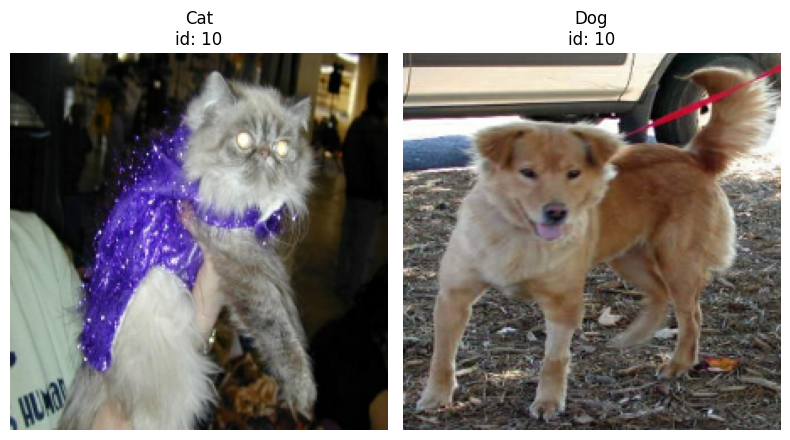
\includegraphics[width=0.6\linewidth]{rysunki/cats&dogs/tested_samples_cats&dogs.png}
    \caption{Zdjęcia badanych próbek do zbioru dotyczącego klasyfikacji psów i kotów [źródło własne]}
    \label{fig:cats&dogs_tested_samples}
\end{figure}